\documentclass{report}
\usepackage[pdftex]{graphicx}
\usepackage[english]{babel}
\usepackage{float}
\begin{document}
\title{Temperature and Humidity Monitoring System}
\author{Jason Pearson, Marcel Englmaier and Justin Koehler}
\maketitle
\tableofcontents
\newpage

\subsection*{Background}
\addcontentsline{toc}{subsection}{Background}
Our client has many needs that have been unmet for various reasons. With problems in their current situation, and our project provides solutions to those needs and to provide resolutions to their problems.
\newline
\indent
  Per Wikipedia, Western Michigan University's (WMU for short) Parkview campus was built in 2003 at a cost of $\$$72.5 million and is the home of the Western Michigan University College of Engineering and Applied Sciences (CEAS for short). 
 WMU’s engineering website explains that WMU has “state-of-the-art resources housed in a $\$$100 million high-tech facility”. 
Sadly, our client has advised that this did not include any automated temperature or humidity sensors and reporting equipment in any of the rooms. 
 These are absolutely critical in rooms that maintain computer, technology, manufacturing, and scientific equipment to safeguard the investment and resources of the university.  There are many risks that computer equipment face as the spent their entire life conducting electricity and being made of rust-prone metals. Standard servers are recommended to be kept at an average temperature of 22°C or less, with automatic shut-off or critical shutdown temperature maximums of 35°C. They must also be kept dry as any condensate will not only short any circuit boards it touches, but cause the servers themselves to rust, as well as the metal racks that support them. Aside from rusts and shorts, excess humidity is a cause of molding and mildewing which is unhealthy for personnel and students, and also damages hardware and clogs air filters. There are many factors that provoke the need for this monitoring, from the downtime of a website, to the security networks that safeguard a campus, the need to have digital phones online, to safeguard data that would be lost in a failure, to the overall cost of the hardware. As an example, one server cluster with the moniker "Thor" has a hardware value of $\$$400,000 which would result in an excessive loss for the university if it were damaged. 
 Our client informed us that there have been several incidences where the temperature of servers increased unhindered to the point that equipment was destroyed due to this lack of automated environment reporting. One such incident where the temperature increased without staff knowing resulted in a ~$\$$500,000 loss. A previous loss due to humidity occurred when the humidity rose to the point of condensation and large steel papermaking rolls generated a layer of surface rust, rendering it unusable until it was repaired or replaced, causing monetary damages and downtime. 
Since the fateful incident, WMU has had students implement several forms of reporting, and currently uses the Temperature @lert WiFi Edition to keep track of the temperature of rooms around campus. 
These sensors work very well but their major flaw is that they are very expensive. These sensors cost upwards of three hundred dollars per sensor and have many features that are neat, but unnecessary for our purposes. 
To alleviate this problem we proposed to create a server that would communicate with a network of home brewed, while reliable sensor computers. 
The server was created by another Western Michigan Computer Science senior design team and it currently is used to communicate with the @lert sensors.
\newline
\indent  
We are unaware at this time of some specific information regarding the facility such as the type and rating of their heating, ventilation, and air conditioning systems (HVAC for short), the dollar value of the equipment lost in the past, the British Thermal Units (BTU’s for short) that are generated by this equipment, or how fast the temperature would increase in the rare event of an HVAC malfunction, but it is clear that their need for automated reporting, and our solution will be more than adequate regardless of this information. Our client has provided us with basic information that due to the thermal mass of the equipment in the rooms, a notification within several minutes would be more than adequate to prevent damage. As our prototype currently stands, there is roughly up to a 3 minute delay before a notification would be sent due to a sixty second temperature fetch cycle from the raspberry pi, a sixty second fetch cycle by the web server, and a sixty second processing cycle that generates the web pages, generates reports, processes data to the database, and would send an alert if the circumstances arose. This could easily be reduced to a total of sixty seconds for the whole process, and very well may be user-selectable on the web page at our client's request. 
It will increase autonomy, provide reporting, reduce cost, add better functionality, 
and provide a product that can be used by students and administrators alike.
\newline
\indent
	The currently used Temperature @lert WiFi sensor has accuracy of $\pm$.$5\,^{\circ}{\rm C}$. The max and minimum temperatures that the current sensor will calculate are -$10\,^{\circ}{\rm C}$ and +$85\,^{\circ}{\rm C}$. 
The current sensor also gives humidity readings. 
This is not high priority, but if we are able to implement it that would be desirable.
 The humidity readings that the current sensors give are between 10$\%$ and 90$\%$ relative humidity. 
This relative humidity has $\pm$ 3$\%$ relative humidity accuracy One major feature of the sensor is the fact that it can be used over the network using wired or wireless connections. 
The wireless specs that it abides by are the 802.11b/g standards and allow for WPA/WEP security. 
These are the features that are used by the system that we need to implement on our client devices.
\newline
\indent
The website that we inherited from the previous team initial page looks like the following figure. 
On this page it shows a graph of all the temperatures that are currently being tracked. 
It does not currently do anything with humidity.  We will be evolving the site to include this information in future releases. 
This uses a framework that allows easy data viewing and little coding. 
We will probably use the same framework to implement this graphing process. 
Once logged in there is much more functionality for the graphing. 
\begin{figure}[H]
\makebox[\textwidth]{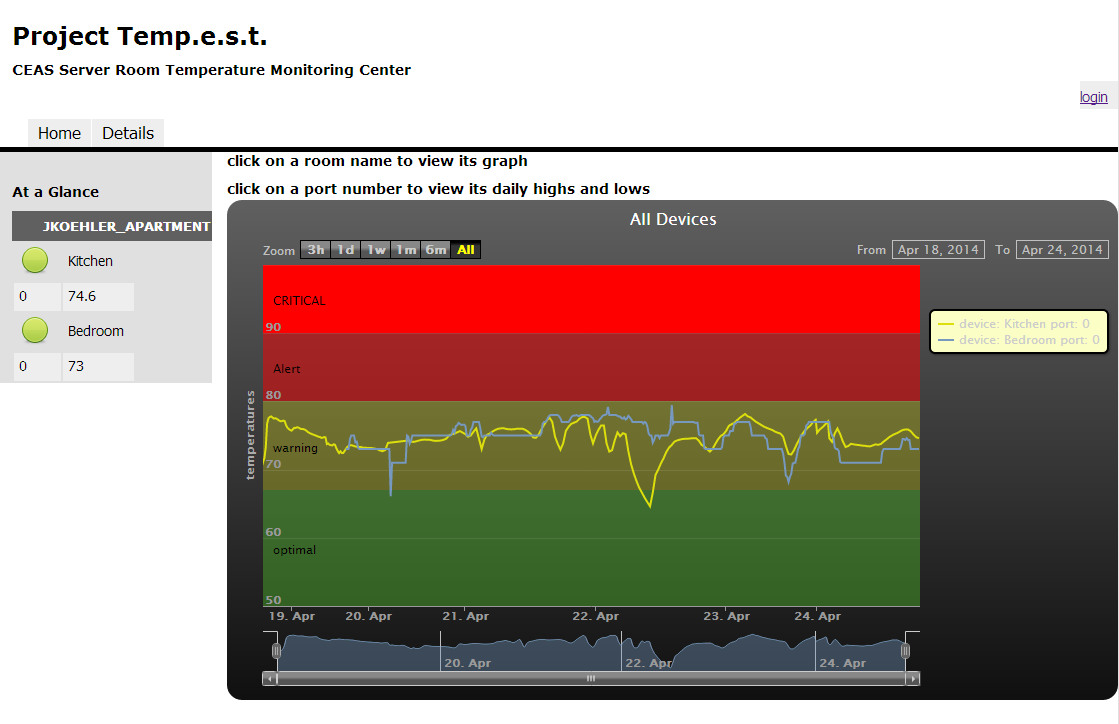
\includegraphics[scale=0.5]{Website.PNG}}
\caption{Initial View Of Site}
\end{figure}
The login process is very basic at this time but in future release will utilize stricter security, data sanitization, and input verification,
and will prevent against session hijacking, network eavesdropping, cross site scripting, and brute force attacks. 
At this time the page will simply have a “Username” and “Password” field (along with a submit button) which will have functionality
added that disables the browser from remembering or saving this information. 
Our first “alpha” release will be using a test database with test users, test usernames, test passwords, and test data, so the security
will not be an issue during this phase. When the user submits, the framework will reference the data to see if it matches what is in the database, and if it does, provide further access to the site, and if not, it will require the user to try again. 
\newline
\indent
There will be only one login page, but based on whether the user successfully authenticates as an administrator or a simple user will determine the pages and views they have access to. 
The admin will have access to the identical pages as the user, but will have an administrator functionality added to the pages, which will allow them to add new users, rooms, and devices, as well as delete or modify existing users, rooms, and devices. 
A regular user will have a list of devices, whereas an administrator will see the same list but will have a button above said list that takes them to an “add device” page.  
The list will have an “edit” and “delete” button next to each device for administrators as well. The edit and delete pages will be similar to the add page, and will be basically the same for users, devices, and rooms. 
\begin{figure}[H]
\makebox[\textwidth]{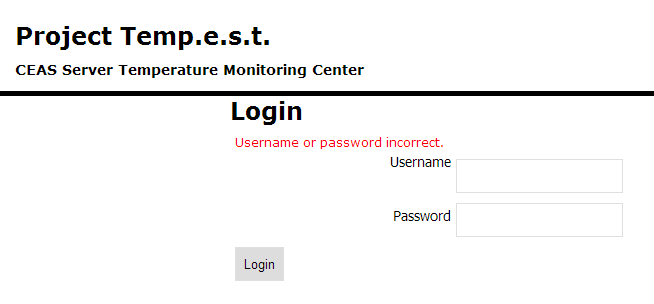
\includegraphics[scale=0.75]{LoginPage.PNG}}
\caption{Login Page}
\end{figure}
\newpage

Upon logging in as a system administrator this is what the admin will see.
This is the general hub for editing anything on the site.
From here the admin can see rooms, users, room assignments and device types easily.
The page looks just the same for a room administrator when logging into the site. 
The only difference is that the room user won't have the option to edit any rooms, devices etc.
If a non logged in user tries to access this page it will redirect them to the login page so that all admin data isn't available to the public.

\begin{figure}[H]
\makebox[\textwidth]{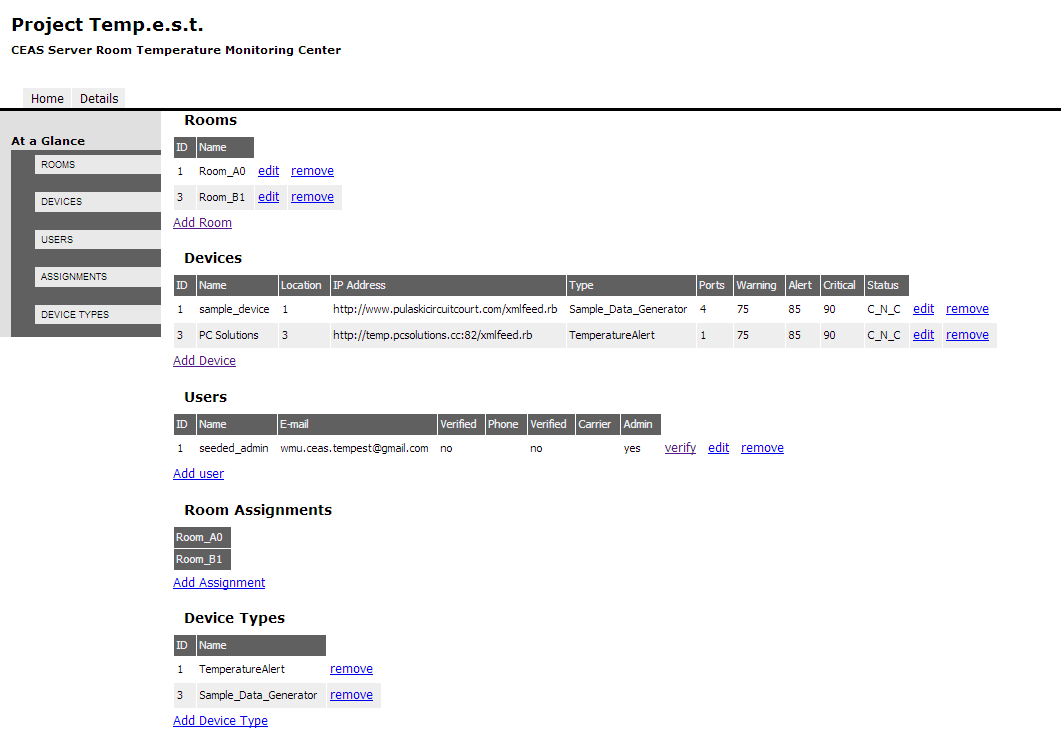
\includegraphics[scale=0.5]{AddPage.PNG}}
\caption{Add Page}
\end{figure}

The following figure is the form used when adding a new device to the network.
The IP address is a major need in this form because it tells the server where to look for the xml. 
The alert and critical thresholds are for when to warn administrators for that room.
The number of ports specifies simply the number of temperatures to expect coming from that device.

\begin{figure}[H]
\makebox[\textwidth]{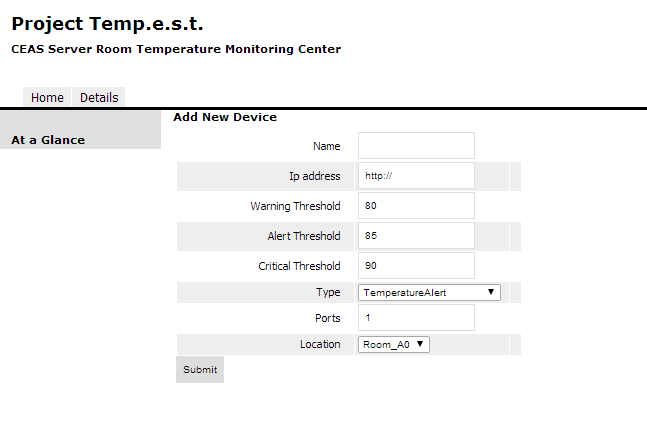
\includegraphics[scale=0.75]{AddDevice.PNG}}
\caption{Add Device To Network Page}
\end{figure}


\begin{figure}[H]
\makebox[\textwidth]{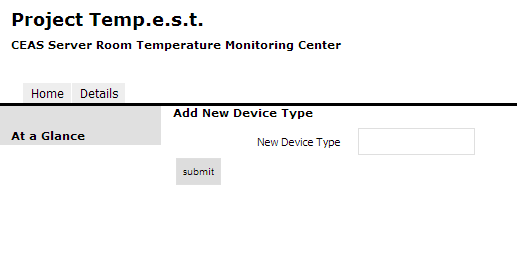
\includegraphics[scale=0.75]{AddDeviceType.PNG}}
\caption{Add Another Device Type}
\end{figure}

The following page is used to add a room to the monitoring system.
The main purpose of a room is to group sensors together and make it easier to distribute work among the administrators.

\begin{figure}[H]
\makebox[\textwidth]{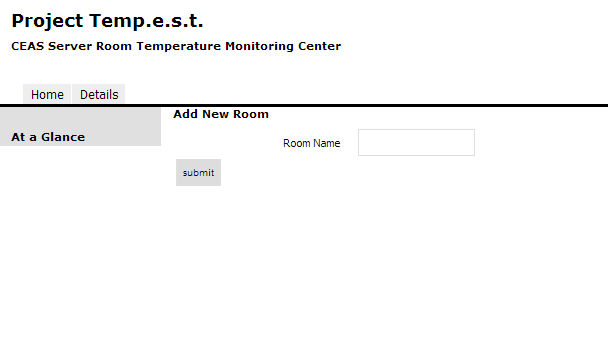
\includegraphics[scale=0.75]{AddRoom.PNG}}
\caption{Adds a Room}
\end{figure}

There are three different levels of users.
The highest level of user is the main system administrator.
This administrator is in control of the whole system. 
Their permissions include but are not limited to adding new users, adding new devices, adding new rooms etc. 
The second tier of user are the normal room administrators.
The room administrators are able see the stats of the rooms they have access and will receive alerts for those rooms.
The last layer of user is the non-registered user. 
This user can see the graph of data on the front page and login. 
It is beneficial to have it this way in case an administrator wants to quick check things and doesn't want to bother with logging in.
Below shows the form for adding a new user. The required fields are name, email, and password. 
The password does have minimal requirements for good passwords.
\begin{figure}[H]
\makebox[\textwidth]{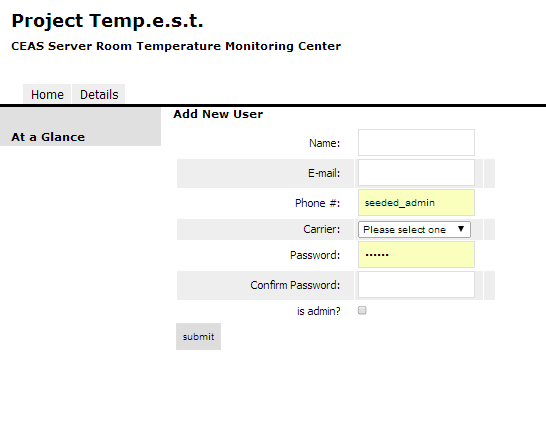
\includegraphics[scale=0.75]{AddUser.PNG}}
\caption{Page To Add Users}
\end{figure}


\begin{figure}[H]
\makebox[\textwidth]{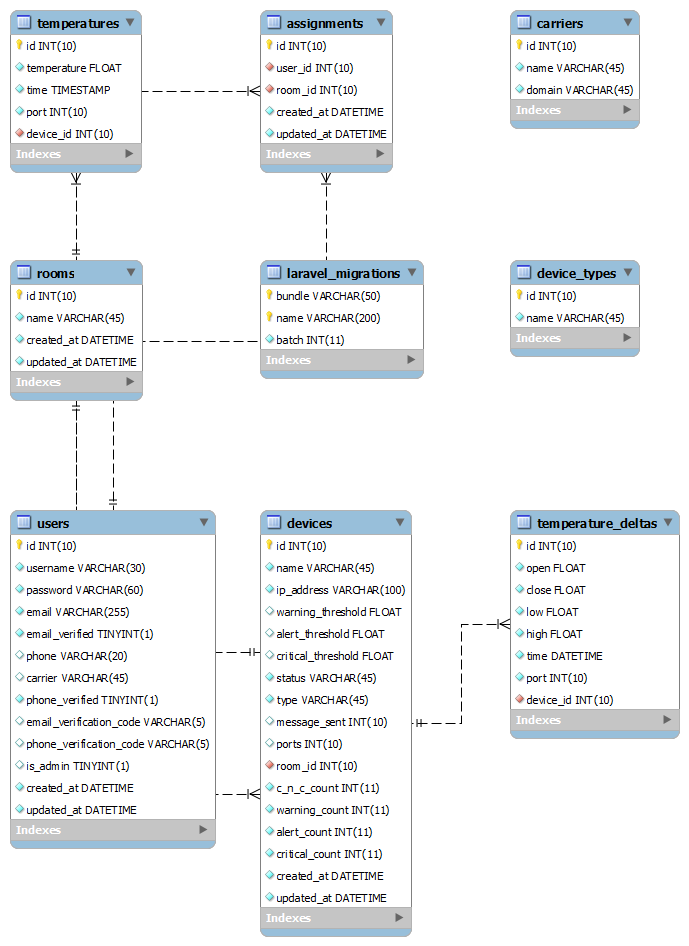
\includegraphics[scale=0.35]{ERDDiagram.png}}
\caption{Entity Relationship Diagram}
\end{figure}

\newpage
\subsection*{Design}
\addcontentsline{toc}{subsection}{Design}

\newpage
\subsection*{Design Decisions}
\addcontentsline{toc}{subsection}{Design Decisions}
	
\newpage
\subsection*{Implementation}
\addcontentsline{toc}{subsection}{Implementation}
\newpage

\subsection*{Testing}
\addcontentsline{toc}{subsection}{Testing}
There are two types of testing that we used in this project unit testing and functional testing. Unit Testing is a must because it will allow the user to test every feature when a new patch comes out and allows after each upgrade to check if the features still work. Unit tests cannot be used to check everything so there must also be functional tests that show the site is reacting correctly and can handle loads properly.
\newline
\indent
Unit tests for this project are ran through the command line and use laravel's testing framework. 
\newline
\indent
There were many different functional tests that we ran to test full functionality of our project. A few tests that we ran include
\begin {itemize}
\item E-mail Alerts
\item Text Message Alerts
\item 
\end {itemize}

\newpage
\subsection*{Security}
\addcontentsline{toc}{subsection}{Security}
\newpage

\subsection*{Maintenance}
\addcontentsline{toc}{subsection}{Security}
\newpage
After the completion of this project the current senior design team will offer no maintenance. All modifications will be done by the staff at Western Michigan University and anyone else who uses the project. This being said there are modifications that we had planned but didn't have time to get to that could be added to increase the user experience for the project. These include
\begin {itemize}
\item Adding a secure layer between the pi and the server
\item Adding historical data logging to the Raspberry Pi
\item Creating a way to retrieve historical data from the device if it was down for a period
\item Upgrading the user control area to have group administration
\item Making a program that would poll servers for their data and add it to a graph
\end {itemize}

\subsection*{Resources}
\addcontentsline{toc}{subsection}{Maintenance}
\newpage

\begin{itemize}
\item Raspberry Pi
\item Temperature Sensors
\item Humidity Sensors
\item Web Server
\item Soldering Equipment
\item Operating System loaded SD Cards with Raspbian
\item Power Connectors for Raspberry pi
\item WiFi Connectors for Raspberry pi
\item External Server to Host Website
\end{itemize}
\newpage


\subsection*{References}
\addcontentsline{toc}{subsection}{References}
For everything raspberry pi we use these sites
\begin{itemize}
\item http://www.raspberrypi.org/
\item http://www.raspbian.org/
\item C Programming 2nd Edition
\item http://www.adafruit.com/
\end{itemize}
For everything web server these are the sites we use
\begin{itemize}
\item http://laravel.com/docs/quick
\item http://www.w3schools.com/
\item http://www.noip.com
\item httpd:apache.org
\item http://www.w3.org
\item http://aws.amazon.com/
\end{itemize}
\newpage
\subsection*{Glossary}
\addcontentsline{toc}{subsection}{Glossary}
\begin{description}
\item [GUI] \hfill \\
Graphical User Interface. The windows a user interacts with.
\item [MSP430] \hfill \\
A 16-bit microcontroller platform made by Texas Instruments.
\item [Raspberry Pi] \hfill \\
 A credit-card-sized single-board computer developed by the Raspberry Pi Foundation.
\item [Arduino] \hfill \\
A series of microcontrollers that are very commonly used for computer to real world communications.
\item [Raspbian] \hfill \\
 A Debian based operating system that we will use for our Raspberry Pi’s
\item [CEAS] \hfill \\
College of Engineering and Applied Sciences at Western Michigan University.
\item [PHP] \hfill \\
A recursive acronym for “PHP Hypertext Preprocessor” - the web programming language being used.
\end{description}
\newpage
\subsection*{Ownership}
\addcontentsline{toc}{subsection}{Ownership}
\begin{description}
\item [Licenses] \hfill \\
Our project will be under several licenses. PHP is a free open source software released under the PHP License.
Laravel is licensed under the MIT license and per the agreement we are “free to modify, distribute and re-publish the source code on the condition that the copyright notices are left intact”.
In the event that our project was used to generate revenue, or be sold as a standalone software package, the license permits us “to incorporate Laravel into any commercial or closed source application”.  
The GNU license and will be open source and will be hosted for all to access and modify as they desire on GitHub.
\item [Intellectual Property (IP)] \hfill \\
As this project is being developed as a Senior Design project for Western Michigan University (WMU) at the direction of Dr. John Kapenga, WMU will retain the intellectual rights to the software.
\item [Non-Disclosure Agreement (NDA)] \hfill \\
No non-disclosure agreement is being used at this time.  The project is maintained on GitHub, which is freely and openly accessible to anyone who wishes to view it, and is thus tracked by search engines such as Google, where it is able to be searched for by anyone on the planet.
\item [Warranty] \hfill \\
A maintenance document has been created for the project. Other than that document and this document no other outside assistance is required by the members of this project.
\end{description}

\end{document}
